% Source for diagram_01.svg — the scope of the course.
% Regenerate with:
%   pdflatex diagram_01.tex && inkscape --export-plain-svg -o diagram_01.svg diagram_01.pdf
\documentclass[tikz,border=4pt]{standalone}
\usepackage{amsmath}
\begin{document}
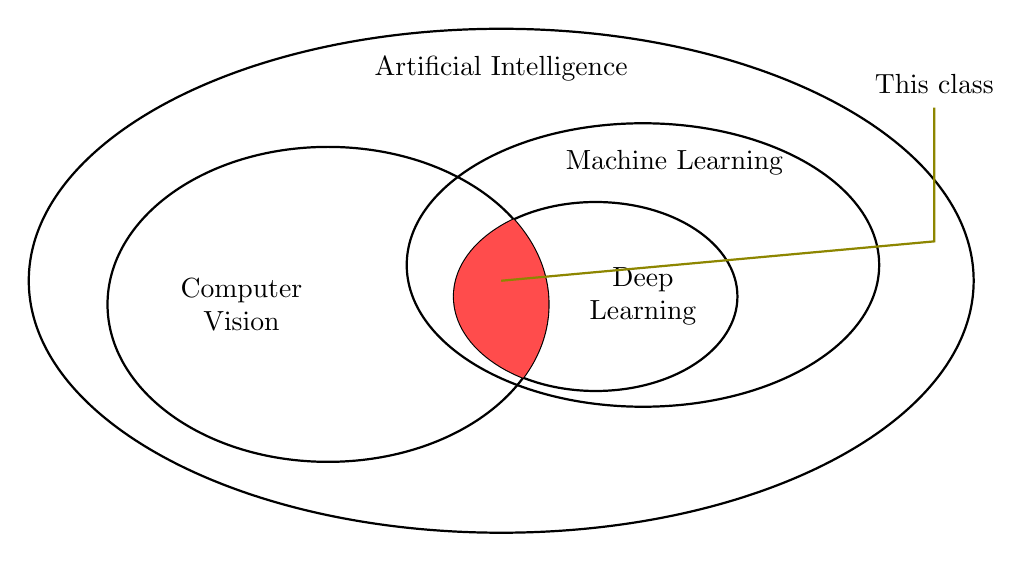
\begin{tikzpicture}[
    every node/.style={font=\normalsize}
]
    % AI - outermost ellipse
    \draw[thick] (0,0) ellipse (6cm and 3.2cm);
    \node at (0, 2.7) {Artificial Intelligence};

    % Computer Vision - LEFT side
    \draw[thick] (-2.2, -0.3) ellipse (2.8cm and 2cm);
    \node[align=center] at (-3.3, -0.3) {Computer\\Vision};

    % Machine Learning - RIGHT side, overlapping with CV
    \draw[thick] (1.8, 0.2) ellipse (3cm and 1.8cm);
    \node at (2.2, 1.5) {Machine Learning};

    % Deep Learning - nested inside ML
    \draw[thick] (1.2, -0.2) ellipse (1.8cm and 1.2cm);
    \node[align=center] at (1.8, -0.2) {Deep\\Learning};

    % Intersection highlight (CV ∩ DL) - red fill
    \begin{scope}
        \clip (-2.2, -0.3) ellipse (2.8cm and 2cm);
        \clip (1.2, -0.2) ellipse (1.8cm and 1.2cm);
        \fill[red!70] (-1, -1.5) rectangle (1, 1.5);
    \end{scope}

    % "This class" label with arrow
    \node[align=center] at (5.5, 2.5) {This class};
    \draw[thick, olive] (5.5, 2.2) -- (5.5, 0.5) -- (0, 0);

\end{tikzpicture}
\end{document}
